%%%%%%%%%%%%%%%%%%%%%%%%%%%%%%%%%%%%%%%%%
% Beamer Presentation
% LaTeX Template
% Version 1.0 (10/11/12)
%
% This template has been downloaded from:
% http://www.LaTeXTemplates.com
%
% License:
% CC BY-NC-SA 3.0 (http://creativecommons.org/licenses/by-nc-sa/3.0/)
%
%%%%%%%%%%%%%%%%%%%%%%%%%%%%%%%%%%%%%%%%%

%----------------------------------------------------------------------------------------
%	PACKAGES AND THEMES
%----------------------------------------------------------------------------------------

\documentclass{beamer}
\usepackage{tikz}
\usepackage{graphicx} % Allows including images
\usepackage{booktabs} % Allows the use of \toprule, \midrule and \bottomrule in tables
\usepackage{ctex}
\usepackage{subfig}
\usepackage{amsmath}
% \usepackage{caption}
% \usepackage{subcaption}

\mode<presentation> {

% The Beamer class comes with a number of default slide themes
% which change the colors and layouts of slides. Below this is a list
% of all the themes, uncomment each in turn to see what they look like.

%\usetheme{default}
%\usetheme{AnnArbor}
\usetheme{Antibes}
%\usetheme{Bergen}
%\usetheme{Berkeley}
%\usetheme{Berlin}
%\usetheme{Boadilla}
%\usetheme{CambridgeUS}
%\usetheme{Copenhagen}
%\usetheme{Darmstadt}
%\usetheme{Dresden}
%\usetheme{Frankfurt}
%\usetheme{Goettingen}
%\usetheme{Hannover}
%\usetheme{Ilmenau}
%\usetheme{JuanLesPins}
%\usetheme{Luebeck}
% \usetheme{Madrid}
%\usetheme{Malmoe}
%\usetheme{Marburg}
%\usetheme{Montpellier}
%\usetheme{PaloAlto}
%\usetheme{Pittsburgh}
%\usetheme{Rochester}
%\usetheme{Singapore}
%\usetheme{Szeged}
%\usetheme{Warsaw}

% As well as themes, the Beamer class has a number of color themes
% for any slide theme. Uncomment each of these in turn to see how it
% changes the colors of your current slide theme.

%\usecolortheme{albatross}
%\usecolortheme{beaver}
%\usecolortheme{beetle}
%\usecolortheme{crane}
%\usecolortheme{dolphin}
%\usecolortheme{dove}
%\usecolortheme{fly}
%\usecolortheme{lily}
%\usecolortheme{orchid}
%\usecolortheme{rose}
%\usecolortheme{seagull}
%\usecolortheme{seahorse}
%\usecolortheme{whale}
%\usecolortheme{wolverine}

%\setbeamertemplate{footline} % To remove the footer line in all slides uncomment this line
%\setbeamertemplate{footline}[page number] % To replace the footer line in all slides with a simple slide count uncomment this line

%\setbeamertemplate{navigation symbols}{} % To remove the navigation symbols from the bottom of all slides uncomment this line
}
\setbeamerfont{caption}{size=\scriptsize}
\setbeamertemplate{caption}[numbered]
\setbeamerfont{footnote}{size=\tiny}
\setbeamerfont{subsection in toc}{size=\small}

% \usepackage{subcaption}

%----------------------------------------------------------------------------------------
%	TITLE PAGE
%----------------------------------------------------------------------------------------

\title[全路网智能路径规划]{电子科技大学本科毕业论文答辩\\全路网智能路径规划} % The short title appears at the bottom of every slide, the full title is only on the title page

\author{董林森} % Your name
\institute[2014070906006] % Your institution as it will appear on the bottom of every slide, may be shorthand to save space
{
电子科技大学,自动化工程学院\\ % Your institution for the title page
\medskip
\textit{lukedong123@gmail.com} % Your email address
}
\date{\today} % Date, can be changed to a custom date

\begin{document}

\begin{frame}
\titlepage % Print the title page as the first slide
\end{frame}

\begin{frame}
\frametitle{大纲} % Table of contents slide, comment this block out to remove it
\tableofcontents % Throughout your presentation, if you choose to use \section{} and \subsection{} commands, these will automatically be printed on this slide as an overview of your presentation
\end{frame}

%----------------------------------------------------------------------------------------
%	PRESENTATION SLIDES
%----------------------------------------------------------------------------------------

%------------------------------------------------
\section{路径规划问题} % Sections can be created in order to organize your presentation into discrete blocks, all sections and subsections are automatically printed in the table of contents as an overview of the talk
%------------------------------------------------

\subsection{数学形式} % A subsection can be created just before a set of slides with a common theme to further break down your presentation into chunks
\begin{frame}
\frametitle{大纲} % Table of contents slide, comment this block out to remove it
\tableofcontents
    [
        currentsection,
        currentsubsection,
        subsectionstyle=show/shaded/hide
    ]
\end{frame}

\begin{frame}
\frametitle{数学形式}
\begin{itemize}

\item 一个有向图定义为$G=(V, E, f)$,其包含一个点集$V = \{1,2,3...n\}$,一个边集$E=\{e_{i,j}| i,j \in V \}$和一个损失函数$f(e_{v_i,v_{i+1}})$。
\item 定义图上的一条路径为$P=\{v_1^P, v_2^P,...,v_k^P\}$,该路径的损失为$L(P) = \sum_{i=1}^{k-1} f(e_{v_i,v_{i+1}})$
\item 最优路径问题:在一个图中,给定起点$S$和终点$E$,求出一条最优路径$P_{optimal}$,使得:
\begin{center}
    \begin{equation}
    P_{optimal} = argmin_{P}(L(P)), v_1^P = S, v_k^P = E
    \end{equation}
\end{center}

\end{itemize}
\end{frame}

\begin{frame}

\frametitle{路径规划问题:数学形式}
\begin{itemize}
    \item 如图\ref{fig:shortespath}所示
\end{itemize}
\begin{figure}
    \centering
    \includegraphics[width=8.0cm]{pic/2-1.pdf}
    \caption{一个最优路径实例(蓝色部分)}
    \label{fig:shortespath}
\end{figure}
\end{frame}

\subsection{基于网格地图的三个场景}
\begin{frame}
\frametitle{大纲} % Table of contents slide, comment this block out to remove it
\tableofcontents
    [
        currentsection,
        currentsubsection,
        subsectionstyle=show/shaded/hide
    ]
\end{frame}

\begin{frame}{网格地图}
\begin{itemize}
    \item 在一个$N\times M$网格地图上,如图\ref{fig:grid}所示。在每个时刻,车辆可以在越过地图的情况下向四个方向移动。
    \item 起点为$S$,终点为$E$。
    \item 网格地图规整的形式有利于强化学习的建模。
\end{itemize}
\begin{figure}
    \centering
    \resizebox{4.0cm}{!}{
        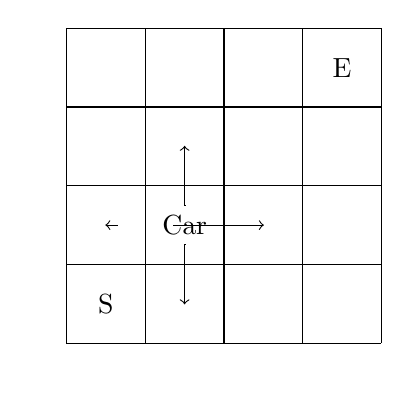
\begin{tikzpicture}[every node/.style={minimum size=1cm-\pgflinewidth, outer sep=0pt}, arrow/.style={thick}]
                \draw[step=1cm,color=black] (-2,-2) grid (2,2); 
                \node[](start) at (-1.5, -1.5) {S};
                \node[](end) at (1.5, 1.5) {E};
                \node[](car) at (-0.5, -0.5) {Car};
                
                \node[](car_up_center) at (0.0, -0.25) {};    
                \node[](car_up) at (-0.5, 1.0) {};
                
                \node[](car_down_center) at (0.0, -0.75) {};
                \node[](car_down) at (-0.5, -2.0){};
            
                \node[](car_left_center) at (-1.35, -0.5) {};
                \node[](car_left) at (-2.0, -0.5){};
            
                \node[](car_right_center) at (-0.65, -0.5) {};
                \node[](car_right) at (1.0, -0.5){};
                
                % \node[](charge site) at (-0.5, 1.5) {$t_{1}$};
                % \node[](charge site) at (1.5, -0.5) {$t_{2}$};
                \draw[->, to path={-| (\tikztotarget)}]
             	( car_up_center) edge (car_up)  (car_down_center) edge (car_down) ;
                 \draw[<-, to path={-| (\tikztotarget)}]
             	(car_left) edge (car_left_center) (car_right) edge (car_right_center);
            \end{tikzpicture}
    }
    \caption{网格地图}
    \label{fig:grid}
\end{figure}
\end{frame}

\begin{frame}{三个路径规划场景}
\begin{itemize}
    \item 场景1,简单网格地图场景,如图\ref{fig:grid}所示,定义每条边上的损失函数$f=C$,$C\geq 0$,为常数。
    \item 场景2,带转弯惩罚的场景,即当车辆左转或掉头,产生额外惩罚$A$,$A\geq 0$,为常数。
    \item 场景3,电动车路径规划场景,车辆电量值$power$最大为$FULL\_POWER$,电量值每次移动减1。地图中加入充电桩${t_1, t_2,...,t_k}$。如图\ref{fig:case3}所示。
\end{itemize}
\begin{figure}
  \centering
      \resizebox{3.0cm}{!}{
            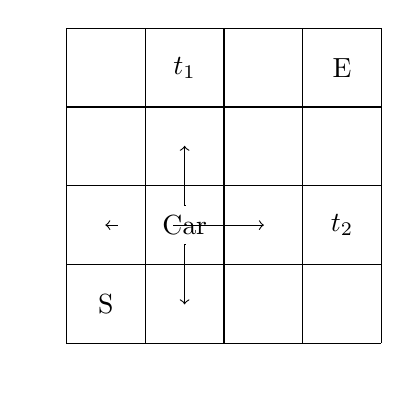
\begin{tikzpicture}[every node/.style={minimum size=1cm-\pgflinewidth, outer sep=0pt}, arrow/.style={thick}]
                    \draw[step=1cm,color=black] (-2,-2) grid (2,2); 
                    \node[](start) at (-1.5, -1.5) {S};
                    \node[](end) at (1.5, 1.5) {E};
                    \node[](car) at (-0.5, -0.5) {Car};
                    
                    \node[](car_up_center) at (0.0, -0.25) {};    
                    \node[](car_up) at (-0.5, 1.0) {};
                    
                    \node[](car_down_center) at (0.0, -0.75) {};
                    \node[](car_down) at (-0.5, -2.0){};
                
                    \node[](car_left_center) at (-1.35, -0.5) {};
                    \node[](car_left) at (-2.0, -0.5){};
                
                    \node[](car_right_center) at (-0.65, -0.5) {};
                    \node[](car_right) at (1.0, -0.5){};
                    
                    \node[](charge site) at (-0.5, 1.5) {$t_{1}$};
                    \node[](charge site) at (1.5, -0.5) {$t_{2}$};
                    \draw[->, to path={-| (\tikztotarget)}]
                 	( car_up_center) edge (car_up)  (car_down_center) edge (car_down) ;
                     \draw[<-, to path={-| (\tikztotarget)}]
                 	(car_left) edge (car_left_center) (car_right) edge (car_right_center);
                \end{tikzpicture}
        } 
    \caption{场景3图示}
    \label{fig:case3}
    \end{figure}
\end{frame}
\section{传统方法:基于图的搜索算法}

\subsection{Dijkstra, $A^*$等传统算算法}
\begin{frame}
\frametitle{大纲} % Table of contents slide, comment this block out to remove it
\tableofcontents
    [
        currentsection,
        currentsubsection,
        subsectionstyle=show/shaded/hide
    ]
\end{frame}

\begin{frame}{Dijkstra 与 $A^*$算法等}
\begin{itemize}
    \item Dijkstra:静态图上的单源最短路,复杂度为$O(|V|^2)$。核心思想在于对每个节点维护一个$D_{v_j}$表示点$v_j$到初始点 $v_s$的距离,并基于松弛操作进行更新。
    \begin{itemize}
        \item $D_{(v_j)} = min(D_{(v_j)}, f(e_{j,k})+ D_{(v_k)})$
    \end{itemize}
    \item $A^*$:启发式搜索方法,每次选出启发式函数值最小的点,并对邻居点进行松弛操作。时间复杂度为多项式级别。
        \begin{itemize}
        \item 启发式函数:$f(v_i) = g(v_i) + h(v_i)$的,$g(v_i)$:从初始点走到 $v_i$的损失值,$h(v_i)$:从点$v_i$到目标点的估计距离(欧几里得距离等)。
        \end{itemize}
    \item 多源最短路算法Floyd,可处理负环的 Bellman-Ford 算法。
\end{itemize}
\end{frame}

\subsection{相关改进算法}
\begin{frame}
\frametitle{大纲} % Table of contents slide, comment this block out to remove it
\tableofcontents
    [
        currentsection,
        currentsubsection,
        subsectionstyle=show/shaded/hide
    ]
\end{frame}
\begin{frame}{相关改进算法}
\begin{itemize}
    \item 基于预处理和查询的分布思想[P. Sanders, D. Schultes, 2001]。
    \item 拆分图为静态拓扑结构和动态损失计算模式,分步处理,使得兼容多种损失函数[D. Delling, A. V. Goldberg, T. Pajor, et al, 2011]。
    \item 对图做简化处理:缩点,分层等思想[P. Sanders, D. Schultes, 2005][R. Geisberger, P. Sanders, D. Schultes, et al, 2008]。
\end{itemize}
\end{frame}
\subsection{基于图的算法局限性}
\begin{frame}
\frametitle{大纲} % Table of contents slide, comment this block out to remove it
\tableofcontents
    [
        currentsection,
        currentsubsection,
        subsectionstyle=show/shaded/hide
    ]
\end{frame}

\begin{frame}{基于图的算法局限性}
% \begin{itemize}
%     \item 基于场景的特殊化方法,通用性低。出现新的场景需要重新设计算法。
%     \begin{itemize}
%         \item 
%     \end{itemize}
%     \item 损失函数的定义有局限性。
%         \begin{itemize}
%             \item 例如倾向选择公共交通方式,不走收费路段等特殊损失函数。
%         \end{itemize}
%     \item 
% \end{itemize}

\begin{block}{通用性}
基于场景的特殊化方法,通用性低。出现新的场景需要重新设计算法。导致出现了基于静态图,动态图,时序依赖的图等各类算法。
\end{block}
\begin{block}{损失函数}
损失函数的形式单一,难以容易多种限制和信息。例如电动车路径规划问题,如何引入行驶路径限制,以及用户倾向选择不同交通方式,不走收费路段等特殊损失函数。
\end{block}
因此需要提出一个具有高通用性和灵活性的框架。
\end{frame}

\section{我们的方法:基于强化学习的算法}

\subsection{强化学习与 Q-Learning}
\begin{frame}
\frametitle{大纲} % Table of contents slide, comment this block out to remove it
\tableofcontents
    [
        currentsection,
        currentsubsection,
        subsectionstyle=show/shaded/hide
    ]
\end{frame}
\begin{frame}{强化学习背景}
    \begin{itemize}
        \item 强化学习(Reinforcement Learning)为一类决策框架
        \begin{itemize}
            \item 广泛应用于博弈论,群体智能等领域,例如战胜围棋世界冠军的 AlphaGo [D.Silver, A.Huang, C.J.Maddison, et al, 2016]
        \end{itemize}
        \item 基于智能体(Agent)建模,并在马尔科夫决策过程(Markov Decision Process, MDP)上进行控制过程,如图所示\ref{fig:RL}
        \item $MDP=(S, A, P(s'| s, a), R(s,a), \gamma)$
    \end{itemize}
    \begin{figure}
    \centering
    \includegraphics[width=8.0cm]{pic/4-1.png}
    \caption{强化学习框架图}
    \label{fig:RL}
\end{figure}
\end{frame}


\begin{frame}{价值函数与策略函数}
\begin{itemize}
    \item 定义策略为$\pi(a|s) = \mathbb{P}[a_t=a | s_t=s]$
    \item 定义状态价值函数为$q_{\pi}(s,a)$为式\ref{eqQvalue},表示以状态$s$作为初始状态,采取行为$a$,然后按照策略$\pi$进行决策下,智能体所受到的累计奖赏值。

        \begin{equation}
            \label{eqQvalue}
            \begin{aligned}
             q_{\pi}(s,a)   & =\mathbb{E}_{\pi}[G_t|s_t=s, a_t=a] \\          
                            & =\mathbb{E}[\sum_{k=0}^{\infty}{\gamma^k{R_{t+k+1}}}|s_t=s, a_t=a]
            \end{aligned}
    \end{equation}
\end{itemize}

\end{frame}

\begin{frame}{Q-Learning}
\begin{itemize}
    \item 最优$Q$值函数$q_{*}(s, a)$,定义为式\ref{Qfunc}。
        \begin{equation}
        \label{Qfunc}
            q_{*}(s, a) = max_{\pi}q_{\pi}(s, a),
            \mbox{for all s $\in$ S and a $\in A_s$.}
        \end{equation}
    \item 基于采样的时序差分方法求解 $q_{*}(s, a)$,且$q_{*}(s, a)$由一个查找表维护:
        \begin{equation}
            Q(s_t, a_t) \leftarrow (1 - \alpha)Q(s_t, a_t) + \alpha[r_{t+1} + \gamma max_{a}Q(s_{t+1}, a)]
        \end{equation}
    
    \item 根据公式\ref{eq4optimalpolicy},由$q_{*}$ 导出最优策略 $\pi_{*}$。
        \begin{equation}
        \pi_{*}(a|s) = \begin{cases}
        1 &\mbox{if $a = argmax_{a \in A_s}q_{*}(s, a)$}\\
        0 &\mbox{else}
        \end{cases}
        \label{eq4optimalpolicy}
        \end{equation}
\end{itemize}
\end{frame}
\subsection{算法设计与系统流程}
\begin{frame}{场景1:简单网格地图}
\begin{itemize}
    \item 对于场景1,奖赏函数设计为\footnote{限于篇幅,不介绍$S$,$A$等的介绍}:
        \begin{center}
           \begin{equation}
            \label{rewardcase1}
            R_t^{case1}(s_t, s_{t+1}, a_t) = \begin{cases}
             sng(Dis(P_{t+1}^{car}, P_{t+1}^{target}) - Dis(P_{t}^{car}, P_{t}^{target}) + A &\\ \mbox{if reach the target}\\
             sng(Dis(P_{t+1}^{car}, P_{t+1}^{target}) - Dis(P_{t}^{car}, P_{t}^{target}) - B &\\ \mbox{if hit bound of map}\\
             sng(Dis(P_{t+1}^{car}, P_{t+1}^{target}) - Dis(P_{t}^{car}, P_{t}^{target}) &\\ \mbox{else}\\
             \end{cases}
            \end{equation} 
        \end{center}

        \item 其中$sng(\cdot)$ 为符号函数, $Dis(\cdot)$ 为欧式距离计算公式
    \item 智能体接近目标点时获得+1的奖赏,反之获得-1的奖赏。
    \item 到达目标点时,给予奖励 $A$。尝试超出地图边界时,给予惩罚$B$。
    
\end{itemize}
\end{frame}
\begin{frame}{场景2:带有转弯惩罚的地图}
    \begin{itemize}
        \item 在场景1的奖赏函数的基础上,加入转弯惩罚\footnote{限于篇幅,不介绍$S$,$A$等的定义}
        \begin{equation}
        \label{eq2reward}
            R_t^{case2}(s_t, s_{t+1}, a_t) = \begin{cases}
             R_{case1}(s_t, s_{t+1}, a_t) - C &\mbox{if turn left or back}\\
             R_{case1}(s_t, s_{t+1}, a_t) &\mbox{else}\\
             \end{cases}
    \end{equation}
    \item 当智能体选择左转或掉头时,给予额外的乘法$C$
    \end{itemize}
\end{frame}

\begin{frame}{场景3:电动车路径规划场景}
\begin{itemize}
    \item 在场景3的设计中,不同于1,2,我们对状态加入了充电桩的坐标$t_1, t_2$,以及剩余电量 $pwoer_t$,以给智能体提供足够的信息用于决策。
    \item 对奖赏函数的设计如下{限于篇幅,不介绍$S$,$A$等的定义}:
        \begin{equation}
        \label{eq3reward}
        R_t^{case3}(s_t, s_{t+1}, a_t) = \begin{cases}
         R_{case1}(s_t, s_{t+1}, a_t) - D &\\ \mbox{if the car out of power in the middle}\\
         R_{case1}(s_t, s_{t+1}, a_t) + E& \\ \mbox{if car reach the charge site}\\
         R_{case1}(s_t, s_{t+1}, a_t)&\\ \mbox{else}
        \end{cases}
    \end{equation}
\end{itemize}
\end{frame}
\begin{frame}
\frametitle{系统流程} % Table of contents slide, comment this block out to remove it
\begin{itemize}
    \item 将算法应用到实际路径规划系统中采用如下的流程图:
    \begin{figure}
        \centering
        \includegraphics[width=7.3cm]{pic/sysmte.pdf}
        \caption{系统流程图}
        \label{fig: system}
    \end{figure}
\end{itemize}
\end{frame}


\section{实现及实现结果}
\subsection{基于面向对象的代码实现}
\begin{frame}
\frametitle{大纲} % Table of contents slide, comment this block out to remove it
\tableofcontents
    [
        currentsection,
        currentsubsection,
        subsectionstyle=show/shaded/hide
    ]
\end{frame}

\begin{frame}{代码设计}
\begin{itemize}
    \item Python 实现。基于面向对象设计。增加代码的灵活性,鲁邦新和可扩展性\footnote{Giuthub 开原地址:http://bit.ly/2kQytSo}。
    \item 智能体表示为 Agent抽象类,环境表示为 Environment抽象类。
    \item 部分特性:
        \begin{itemize}
            \item 设计 Config 类,托管所有参数,解除硬编码(Hard Code)
            \item 自动化的统计训练过程数据
            \item 基于设计模式的策略模式(Strategy Pattern),分离算法模型(Model)和智能体,
        \end{itemize}
    \item 工作量:源代码约5000行。
\end{itemize}
\end{frame}

\subsection{实验结果}

\begin{frame}
\frametitle{大纲} % Table of contents slide, comment this block out to remove it
\tableofcontents
    [
        currentsection,
        currentsubsection,
        subsectionstyle=show/shaded/hide
    ]
\end{frame}

\begin{frame}{实验设置}
    \begin{itemize}
        \item 相同参数下,使用不同随机种子,进行10次独立实验,数据求平均。
        \item 地图大小为 $4\times 4$
        \item 智能体采样100个数据样本后进行一次训练,然后进行一次测试,测试时采样100个数据样本进行评估。
        \item 训练迭代次数,以及学习速率参数各个场景单独调试。
        \item 可视化测试时智能体的累计奖赏值曲线和部分状态下的 Q 值以展示结果。
    \end{itemize}
\end{frame}

\begin{frame}{场景1:累计奖赏值曲线}
    \begin{itemize}
        \item 累计奖赏值随训练迭代次数变化曲线如图\ref{fig:case1}。
    \end{itemize}
\begin{figure}
    \centering
    \includegraphics[width=6.0cm]{pic/case1/case1.pdf}
    \caption{测试下的累计奖赏曲线,虚化部分为10次试验统计方差上下界}
    \label{fig:case1}
\end{figure}
\end{frame}

\begin{frame}{场景1:Q 值变化曲线}
    \begin{itemize}
        \item 点(0,0),向上和向右为最优行为;点(3,0),向上为最优行为;点(0,3),向右为最优行为。
    \end{itemize}
    \begin{figure}
      \centering
      \subfloat[(0,0)点\label{fig:00}]{\includegraphics[width=3.0cm]{pic/case1/00.pdf}}\qquad
      \subfloat[(3,0)点\label{fig:00}]{\includegraphics[width=3.0cm]{pic/case1/30.pdf}}\qquad
      \subfloat[(0,3)点\label{fig:00}]{\includegraphics[width=3.0cm]{pic/case1/03.pdf}}\qquad
    \caption{各点$Q$值变化曲线}
    \label{figcase1Q}
    \end{figure}
\end{frame}

\begin{frame}{场景2:累计奖赏值曲线}
    \begin{itemize}
        \item 累计奖赏值随训练迭代次数变化曲线如图\ref{fig:case2}。
    \end{itemize}
\begin{figure}
    \centering
    \includegraphics[width=6.0cm]{pic/case2/case1.pdf}
    \caption{测试下的累计奖赏曲线}
    \label{fig:case2}
\end{figure}
\end{frame}

\begin{frame}{场景2:Q 值变化曲线}
    \begin{itemize}
        \item 点(0,0),向上(避免左转)为最优行为;
        \item 当在点(3,0),且上一时刻方向为向右时,智能体仍然选择左转到达目标点,说明智能体的策略使得在保证经过最短路径的情况下减少左转,如图\ref{fig:00}所示。
    \end{itemize}
    \begin{figure}
      \centering
      \subfloat[(0,0)点\label{fig:00}]{\includegraphics[width=4.2cm]{pic/case2/00.pdf}}\qquad
      \subfloat[(3,0)点\label{fig:00}]{\includegraphics[width=4.2cm]{pic/case2/303.pdf}}\qquad
    \caption{各点$Q$值变化曲线}
    \label{fig:case2qvalue}
    \end{figure}
\end{frame}

\begin{frame}{场景3:累计奖赏值曲线}
    \begin{itemize}
        \item 累计奖赏值随训练迭代次数变化曲线如图\ref{fig:case3}。
    \end{itemize}
\begin{figure}
    \centering
    \includegraphics[width=6.0cm]{pic/case3/case1.pdf}
    \caption{测试下的累计奖赏曲线}
    \label{fig:case3}
\end{figure}
\end{frame}

\begin{frame}{场景3:Q 值变化曲线}
    \begin{itemize}
        \item 检测当仅剩1个电量时,智能体能否寻找最近的充电桩\footnote{充电桩位置为(1,2),(3,1)}。
        \begin{itemize}
            \item 在点(1,1)时选择向上到达(1,2)点的充电桩
            \item 在点(2,1)时选择向右到达(3,1)点的充电桩
        \end{itemize}
    \end{itemize}
    \begin{figure}
      \centering
      \subfloat[(0,0)点\label{fig:00}]{\includegraphics[width=4.2cm]{pic/case3/1,1,1.pdf}}\qquad
      \subfloat[(3,0)点\label{fig:00}]{\includegraphics[width=4.2cm]{pic/case3/2,1,1.pdf}}\qquad
    \caption{各点$Q$值变化曲线}
    \label{fig:case3qvalue}
    \end{figure}
\end{frame}

\begin{frame}{场景3:Q 值变化曲线}
    \begin{itemize}
        \item 类似场景2,我们检测特殊点(3,2),即当智能体剩余1个电量时,但距离目标点只有1个格点时,是否会选择正确的行为。
        \begin{itemize}
            \item 向上到达终点(3,3),向下到达(3,1)充电桩。
        \end{itemize}
    \end{itemize}
    \begin{figure}
      \centering
      \includegraphics[width=6.0cm]{pic/case3/3,2,1.pdf}
    \caption{(3,2)点 Q 值变化曲线}
    \label{fig:case2qvalue}
    \end{figure}
\end{frame}

\section{总结与展望}
\subsection{总结}
\begin{frame}
\frametitle{大纲} % Table of contents slide, comment this block out to remove it
\tableofcontents
    [
        currentsection,
        currentsubsection,
        subsectionstyle=show/shaded/hide
    ]
\end{frame}
\begin{frame}{总结}
    在我们的工作中,我们提出了基于强化学习的路径规划算法。主要贡献为:
    \begin{itemize}
        \item 给出了用于端到端的强化学习的路径规划数学模型。
        \begin{itemize}
            \item 通过奖赏函数的设计嵌入原问题的损失函数带来了巨大的灵活性。
        \end{itemize}
        \item 给出了基于 Q-Learnig 的路径规划算法,并解决了两个传统模型难以解决的场景。
        \item 设计并实现了一个具有高灵活性和鲁邦新的代码框架。
    \end{itemize}
\end{frame}

\subsection{后续工作展望}
\begin{frame}
\frametitle{大纲} % Table of contents slide, comment this block out to remove it
\tableofcontents
    [
        currentsection,
        currentsubsection,
        subsectionstyle=show/shaded/hide
    ]
\end{frame}
\begin{frame}{后续工作展望}
    \begin{itemize}
        \item 如何解决大规模地图下的路径规划问题
        \begin{itemize}
            \item 查表法的内存开销过大
            \item 应用深度强化学习(Deep Reinforcement Learning)方法,使用神经网络对 Q 值函数进行拟合。

        \end{itemize}
        \item 如何设计离线算法,单次询问给出全部规划结果。
        \item 如何合理处理仿真环境带来的仿真误差和使用真实环境数据。
        \begin{itemize}
            \item 为此,与指导老师郭宏亮老师进行了相关研究工作。并做了题为 Intelligent Trainer for Model-Based Reinforcement Learning 的论文
            \item 论文已投 NIPS (Conference on Neural Information Processing Systems)\footnote{机器学习领域顶级会议之一} 2018,在审。
        \end{itemize}
    \end{itemize}
\end{frame}

% %------------------------------------------------

% \begin{frame}
% \frametitle{Multiple Columns}
% \begin{columns}[c] % The "c" option specifies centered vertical alignment while the "t" option is used for top vertical alignment

% \column{.45\textwidth} % Left column and width
% \textbf{Heading}
% \begin{enumerate}
% \item Statement
% \item Explanation
% \item Example
% \end{enumerate}

% \column{.5\textwidth} % Right column and width
% Lorem ipsum dolor sit amet, consectetur adipiscing elit. Integer lectus nisl, ultricies in feugiat rutrum, porttitor sit amet augue. Aliquam ut tortor mauris. Sed volutpat ante purus, quis accumsan dolor.

% \end{columns}
% \end{frame}

% %------------------------------------------------
% %------------------------------------------------

% \begin{frame}
% \frametitle{Table}
% \begin{table}
% \begin{tabular}{l l l}
% \toprule
% \textbf{Treatments} & \textbf{Response 1} & \textbf{Response 2}\\
% \midrule
% Treatment 1 & 0.0003262 & 0.562 \\
% Treatment 2 & 0.0015681 & 0.910 \\
% Treatment 3 & 0.0009271 & 0.296 \\
% \bottomrule
% \end{tabular}
% \caption{Table caption}
% \end{table}
% \end{frame}

% %------------------------------------------------

% \begin{frame}
% \frametitle{Theorem}
% \begin{theorem}[Mass--energy equivalence]
% $E = mc^2$
% \end{theorem}
% \end{frame}

% %------------------------------------------------

% \begin{frame}[fragile] % Need to use the fragile option when verbatim is used in the slide
% \frametitle{Verbatim}
% \begin{example}[Theorem Slide Code]
% \begin{verbatim}
% \begin{frame}
% \frametitle{Theorem}
% \begin{theorem}[Mass--energy equivalence]
% $E = mc^2$
% \end{theorem}
% \end{frame}\end{verbatim}
% \end{example}
% \end{frame}

% %------------------------------------------------

% \begin{frame}
% \frametitle{Figure}
% Uncomment the code on this slide to include your own image from the same directory as the template .TeX file.
% %\begin{figure}
% %\includegraphics[width=0.8\linewidth]{test}
% %\end{figure}
% \end{frame}

% %------------------------------------------------

% \begin{frame}[fragile] % Need to use the fragile option when verbatim is used in the slide
% \frametitle{Citation}
% An example of the \verb|\cite| command to cite within the presentation:\\~

% This statement requires citation \cite{p1}.
% \end{frame}

% %------------------------------------------------

% \begin{frame}
% \frametitle{References}
% \footnotesize{
% \begin{thebibliography}{99} % Beamer does not support BibTeX so references must be inserted manually as below
% \bibitem[Smith, 2012]{p1} John Smith (2012)

% \newblock Title of the publication
% \newblock \emph{Journal Name} 12(3), 45 -- 678.
% \end{thebibliography}
% }
% \end{frame}

% %------------------------------------------------

% \begin{frame}
% \Huge{\centerline{The End}}
% \end{frame}

%----------------------------------------------------------------------------------------

\end{document}